%%%%%%%%%%%%%%%%%%%%%%%%%%%%%%%%%%%%%%%%%%%%%%%%%%%%%%%%%%%%%%%%%%%%%%%%%%%
%%  Project: CPHOS LaTeX Template
%%  File: example-problem.tex
%%  Copyright © 2026 gameswu & CPHOS (www.cphos.cn)
%%
%%  Permission is hereby granted, free of charge, to any person obtaining a 
%%  copy of this software and associated documentation files (the "Software"), 
%%  to deal in the Software without restriction, including without limitation 
%%  the rights to use, copy, modify, merge, publish, distribute, sublicense, 
%%  and/or sell copies of the Software, and to permit persons to whom the 
%%  Software is furnished to do so, subject to the following conditions:
%%
%%  The above copyright notice and this permission notice shall be included 
%%  in all copies or substantial portions of the Software.
%%
%%  THE SOFTWARE IS PROVIDED "AS IS", WITHOUT WARRANTY OF ANY KIND, EXPRESS 
%%  OR IMPLIED, INCLUDING BUT NOT LIMITED TO THE WARRANTIES OF MERCHANTABILITY, 
%%  FITNESS FOR A PARTICULAR PURPOSE AND NONINFRINGEMENT. IN NO EVENT SHALL 
%%  THE AUTHORS OR COPYRIGHT HOLDERS BE LIABLE FOR ANY CLAIM, DAMAGES OR OTHER 
%%  LIABILITY, WHETHER IN AN ACTION OF CONTRACT, TORT OR OTHERWISE, ARISING 
%%  FROM, OUT OF OR IN CONNECTION WITH THE SOFTWARE OR THE USE OR OTHER 
%%  DEALINGS IN THE SOFTWARE.
%%%%%%%%%%%%%%%%%%%%%%%%%%%%%%%%%%%%%%%%%%%%%%%%%%%%%%%%%%%%%%%%%%%%%%%%%%%

% CPHOS理论命题模板

\documentclass[answer]{cphos}

% === 设置文档信息 ===
\cphostitle{CPHOS物理竞赛联考}
\cphossubtitle{理论试题命题模板}
% \cphoswatermark{assets/watermark.jpg}  % 可选：自定义水印文件

\enablescorecheck  % 启用分值检查

\begin{document}
\begin{problem}{一}{XX}{这里可以是一个帅气的题目，但是也可以没有} % TODO: 修改分值、标题

% === 题干 ===
\begin{problemstatement}
% TODO: 修改题干内容
这是题目开始之前的一段话（如果有的话）。题目中所有的汉字应使用宋体、五号，此处需要缩进两格。汉字中以及题目编号中的括号均使用中文的标点符号。

题目中的英文单词（非变量或常量）以及数字应使用Times New Roman字体、五号。英文句子中的逗号和句号后应当有一个英文空格，主要是为了美观，如：To be or not to be, that's a question.

文字之中的公式、字母（变量、常量）均使用\LaTeX，如$U=IR$。若公式或需要带入的数据较长，可以使用行间公式，如（公式详尽的注意事项见解答部分）
\begin{equation}
    \int \sqrt{\frac{x}{1-x}} \mathrm{d}x = - \sqrt{x(1-x)} - \arccos{\sqrt{x}} + \mathrm{Const}. \eqtag{1}
\end{equation}

\subq{1} 你可以使用\texttt{\textbackslash subq\{编号\}}、\texttt{\textbackslash subsubq\{编号\}}等命令来标记小问，编号会自动生成并且已经自动设置为无缩进。
\subq{2} 第二问的背景介绍，一级标题。
\subsubq{2.1} 这是二级标题，无缩进。
\subsubq{2.2} 图片不宜过大，图片可以放置在文字右边，或单独成行居中显示。图片统一使用软件AxGlyph绘制，请提供AxGlyph源文件以方便修改。注意通过\texttt{\textbackslash caption\{题注\}}添加题注（题注编号是自动生成的）并设置\texttt{\textbackslash label\{标签\}}，这样可以通过\texttt{\textbackslash ref\{标签\}}引用，例如图\ref{fig:example}。AxGlyph官网为：\url{https://www.amyxun.com}

\begin{figure}[H]
    \centering
    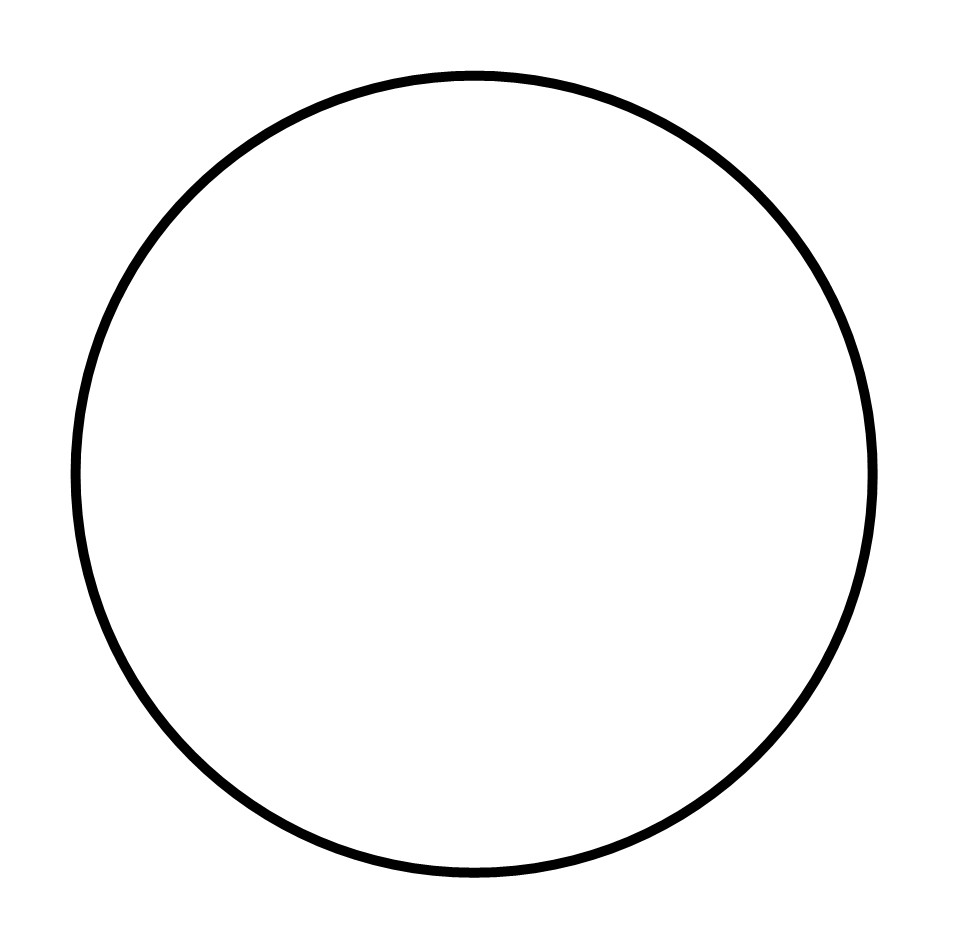
\includegraphics[width=0.4\textwidth]{examples/example.jpg}
    \caption{这是一个示例图片}
    \label{fig:example}
\end{figure}

\noindent 提示，你可能会用到以下公式：这里是题目的提示，在这里你需要使用\texttt{\textbackslash noindent}以去掉自动缩进。
\end{problemstatement}

% === 解答 ===
\begin{solution}
% TODO: 修改解答内容
% 你可以使用\eqtagscore{编号}{分数}来标记公式分值，使用\addtext{说明文字}{分数}来添加非公式分值
% 你需要使用\scorepart{编号}{分数}来标记每个大问的总分，编号需要与题干中的题号一致
\scorepart{1}{15}
（1）这里是一级标题。\ref{eq:1.1}式作为计分公式应单独占一行，你应该使用\texttt{equation}环境来输入，并且在公式末尾使用\texttt{\textbackslash eqtagscore\{编号\}\{分数\}}来标记分值，例如：
\begin{equation}
    F = ma \eqtagscore{1}{3} \label{eq:1.1}
\end{equation}

值得注意的是，我们在上述公式中使用了\texttt{\textbackslash label\{eq:1.1\}}来标记公式，这样你就可以在解答的其他部分通过\texttt{\textbackslash ref\{eq:1.1\}}来引用这个公式，例如式\ref{eq:1.1}。

下面是三角函数和双曲函数的写法，函数用正体，拉丁字母、希腊字母均用斜体。一般的大写希腊字母不是斜体，需要使用\texttt{\textbackslash var}前缀的命令，例如\texttt{\textbackslash varOmega}，来得到斜体的大写希腊字母$\varOmega$。
\begin{equation}
    \cos \phi = \varOmega \sinh \theta \eqtagscore{2}{3}
\end{equation}

常见的数学记号也有专门的命令，例如\texttt{\textbackslash int}、\texttt{\textbackslash sum}、\texttt{\textbackslash lim}、{\textbackslash max}等。特殊常数如自然对数的底$\mathrm{e}$、圆周率$\uppi$、虚数单位$\mathrm{i}$也都应使用正体，分别对应的命令为\texttt{\textbackslash mathrm\{e\}}、\texttt{\textbackslash uppi}、\texttt{\textbackslash mathrm\{i\}}。如 \ref{eq:1.3}式和\ref{eq:1.4}式所示：

\begin{equation}
    \ln p = \exp (-\delta) = \lim_{n \to \infty} \left( 1 - \frac{\delta}{n} \right)^n \eqtagscore{3}{3} \label{eq:1.3}
\end{equation}
\begin{equation}
    a = \max_{0\leq x \leq 1} x \cdot 2^{-x^2} \eqtagscore{4}{3} \label{eq:1.4}
\end{equation}

接下来\ref{eq:1.5}式是积分式的写法，微分符号$\mathrm{d}$使用正体\texttt{\textbackslash mathrm\{d\}}，$\mathrm{Const}.$使用正体\texttt{\textbackslash mathrm\{Const\}.}，也可以直接写$C$。
\begin{equation}
    \int \sqrt{\frac{x}{1-x}} \mathrm{d}x = - \sqrt{x(1-x)} - \arccos{\sqrt{x}} + \mathrm{Const}. \eqtagscore{5}{3} \label{eq:1.5}
\end{equation}

对于答案中插入的图片，处理方式与题干中的图片相同。
\begin{figure}[H]
    \centering
    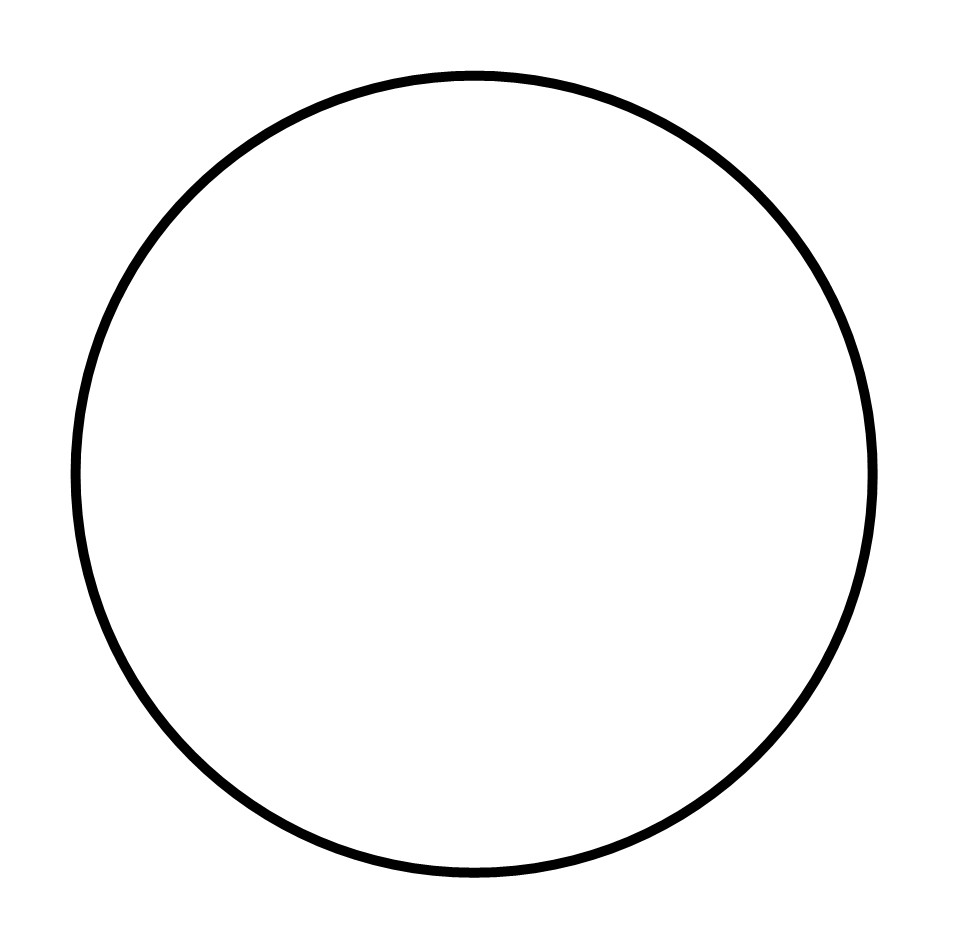
\includegraphics[width=0.3\textwidth]{examples/example.jpg}
    \caption{解答中的示例图片}
    \label{fig:solution-example}
\end{figure}

\scorepart{2}{25}
\scoresubpart{2.1}{10}
（2）（2.1）这是二级标题，\ref{eq:2.1.1}式是角标的用法。矢量统一使用上标箭头\texttt{\textbackslash vec\{\}}而不是加粗，方便观察；平均使用\texttt{\textbackslash bar\{\}}，一般而言，角标等不被包含在平均号和矢量箭头下面，主要是为了美观。
\begin{equation}
    \bar{s}_0 = \vec{v}_1 = a' \eqtagscore{6}{6} \label{eq:2.1.1}
\end{equation}

对于文字说明类的给分，你可以使用\texttt{\textbackslash addtext\{说明文字\}\{分数\}}来标记，例如：
\addtext{讨论}{4}

\scoresubpart{2.2}{15}
（2.2）这也是二级标题，小球质量$m$等物理量作为行内公式使用斜体。一些特别的角标，如$c_{\max}$之类，可以用正体。
\begin{equation}
    M = I\omega \eqtagscore{7}{6}
\end{equation}
\begin{equation}
    E = mc^2 \eqtagscore{8}{6}
\end{equation}

数值和单位之间需要一个空格的间隔（主要也是为了美观），单位使用正体。使用\texttt{\textbackslash text\{\textasciitilde 单位\}}即可。
\begin{equation}
    v = 1.234 \text{~m/s} \eqtagscore{9}{3}
\end{equation}
一些物理常量使用的字母有统一要求，例如对于介电常量应使用$\varepsilon$而不是$\epsilon$。

评分标准现在将自动生成在解答部分的最后，如果你的分值标记不正确的话将会生成提示信息在评分标准部分。

% === 参考文献（可选） ===
\begin{problemreferences}[这里可以写一段简短的说明，也可以什么都不写。后续跟上参考文献，建议遵循ACS style进行标注，并在必要时以上标\supercite{1}引用，引用命令为\texttt{\textbackslash supercite\{num\}}。]
\refitem{Last Name, First Initial.; Last Name, First Initial. ``Title''. \textit{Journal},\textbf{Year}, Volume(issue), Pages.}
\end{problemreferences}

\scoring{40} % TODO: 修改评分标准生成部分的总分
\end{solution}

% === 题目附录（可选） ===
\begin{problemappendix}
\noindent（1）附录内依然可以插入公式并仍然遵循前述公式的格式要求，但是编号不做要求。
\begin{equation*}
    F = ma
\end{equation*}
\noindent（2）善用AI和网络资源快速熟练地掌握\LaTeX 的使用！该模板无法涵盖所有的\LaTeX 细节，但你可以通过网络资源和AI工具来解决使用过程中遇到的任何问题。
\end{problemappendix}

\end{problem}

\end{document}
